\documentclass[aspectratio=169,11pt]{beamer}
\usetheme[progressbar=frametitle]{metropolis}
\usepackage{graphicx}
\usepackage{tikz}
\usepackage{array}
\usetikzlibrary{positioning,shapes.geometric}
\graphicspath{{figures/}}

\definecolor{llblue}{HTML}{1F5F8B}
\definecolor{llorange}{HTML}{E07B24}
\setbeamercolor{progress bar}{fg=llorange}
\setbeamercolor{frametitle}{bg=llblue}
\setbeamercolor{alerted text}{fg=llorange}

\title{AIT Lablink}
\subtitle{Connecting lab hardware, simulators and tools}
\author{}
\date{}
\titlegraphic{\vspace*{-0.6cm}\hfill
\includegraphics[height=1.2cm]{logo_lablink.png}}

\begin{document}

\maketitle

% ---------------------------------------------------------------- 1 Hook
\begin{frame}{How do you do this today?}
  \begin{columns}[T]
    \column{0.55\textwidth}
    \begin{itemize}
      \item Coupling a device under test to a \alert{simulator}
      \item \alert{Logging} measurements from several devices at once
      \item \alert{Repeating} the same test case next week \dots\ or next year
      \item Swapping one device for another without rewiring everything
    \end{itemize}
    \column{0.4\textwidth}
    \vspace{0.6cm}
    \begin{block}{Typical result}
      One-off scripts, manual steps, and setups that are hard to reproduce.
    \end{block}
  \end{columns}
\end{frame}

% ---------------------------------------------------------------- 2 What is it
\begin{frame}{Lablink in one sentence}
  \centering
  \Large
  A common framework that \alert{loosely couples}\\
  lab hardware, simulators and tools\\
  so they can \alert{exchange data}.
  \vspace{1cm}

  \normalsize
  \begin{columns}[T]
    \column{0.3\textwidth}\centering
    \textbf{Couple}\\ components
    \column{0.3\textwidth}\centering
    \textbf{Log}\\ results
    \column{0.3\textwidth}\centering
    \textbf{Automate}\\ test cases
  \end{columns}
  \vspace{0.8cm}

  \small Open source, developed by AIT Austrian Institute of Technology
\end{frame}

% ---------------------------------------------------------------- 3 Architecture
\begin{frame}{The big picture}
  \begin{columns}[c]
    \column{0.62\textwidth}
    \centering
    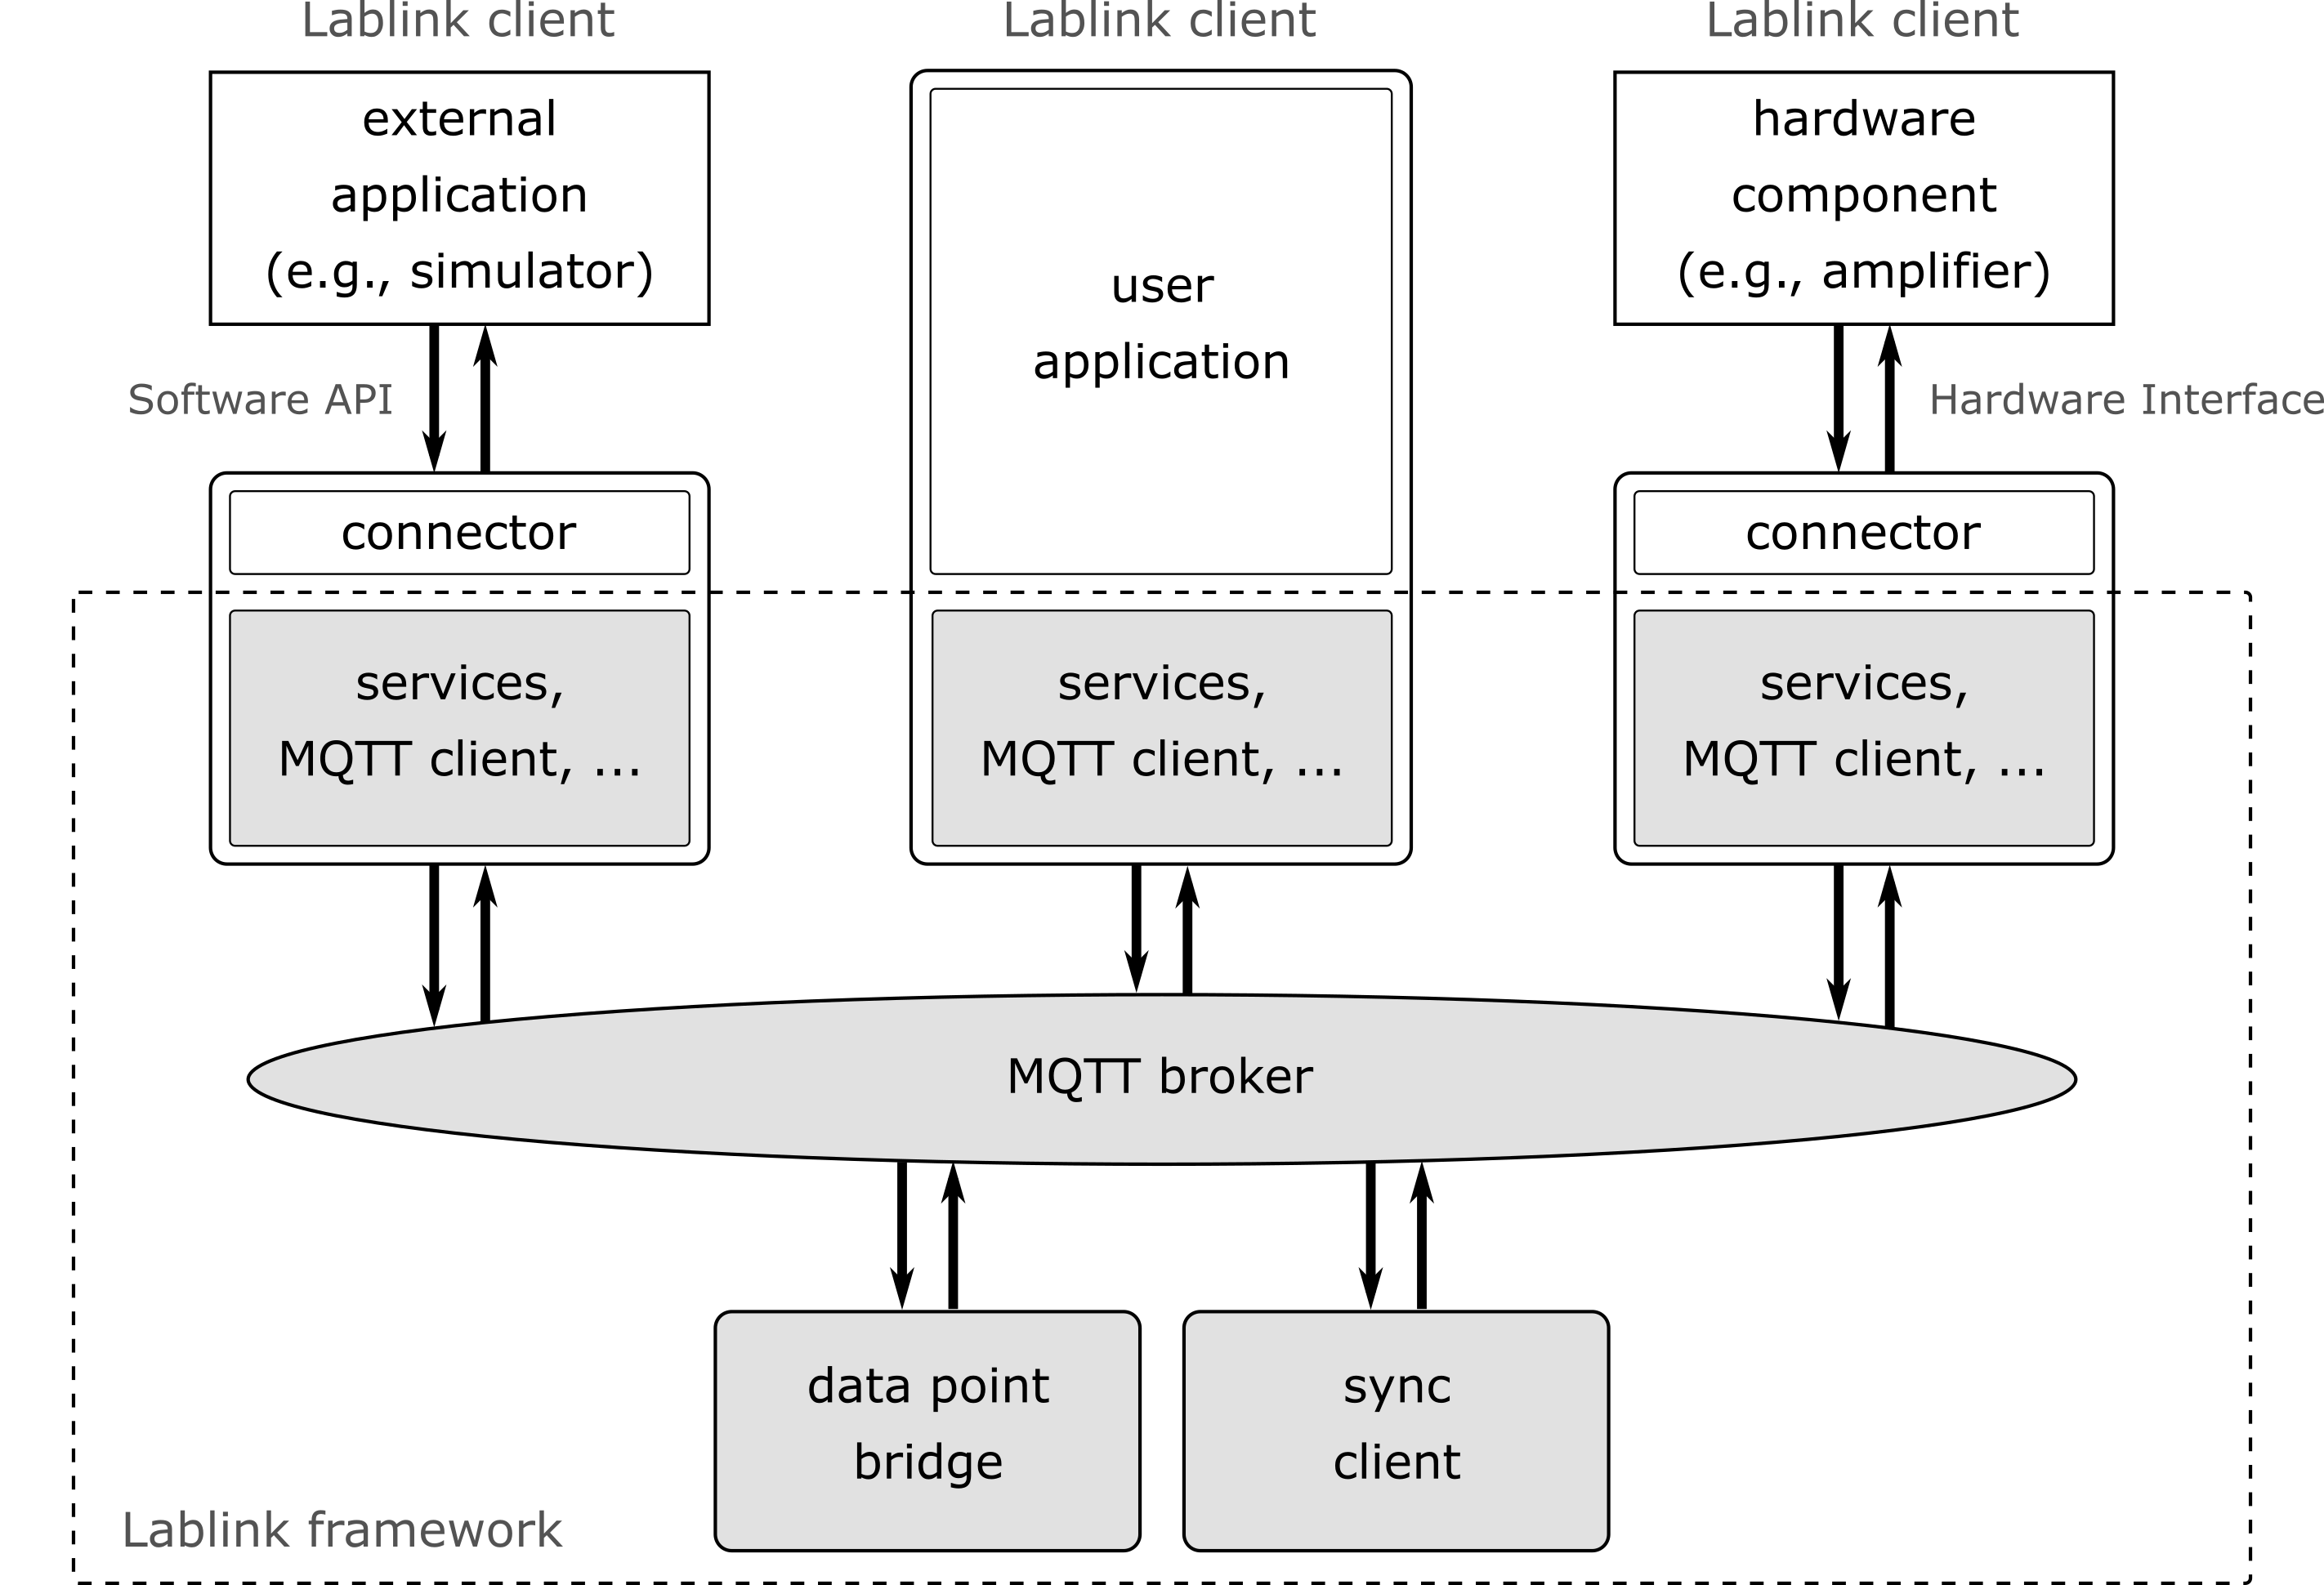
\includegraphics[width=\linewidth]{lablink-architecture.png}
    \column{0.36\textwidth}
    \small
    \begin{itemize}
      \item \textbf{Lablink Core}: the shared communication layer
      \item \textbf{Broker}: distributes all messages (MQTT)
      \item \textbf{Clients}: each has exactly \alert{one} connection
    \end{itemize}
  \end{columns}
\end{frame}

\begin{frame}{Three kinds of clients}
  \begin{columns}[T]
    \column{0.32\textwidth}
    \begin{block}{Simulator connector}
      Links a simulation tool, e.g.\ PowerFactory, to the rest of the setup.
    \end{block}
    \column{0.32\textwidth}
    \begin{block}{Hardware connector}
      Talks to a lab device via standard interfaces, e.g.\ Modbus TCP or serial.
    \end{block}
    \column{0.32\textwidth}
    \begin{block}{Stand-alone client}
      Contains its own logic, e.g.\ a controller or a test sequence.
    \end{block}
  \end{columns}
  \vspace{0.8cm}
  \centering
  Every component looks the same to the rest of the system,\\
  so it can be \alert{replaced} without touching the others.
\end{frame}

% ---------------------------------------------------------------- 4 Communication
\section{How components talk}

\begin{frame}{Three ways to talk}
  \centering
  \renewcommand{\arraystretch}{1.5}
  \small\begin{tabular}{>{\raggedright}p{2.4cm}>{\raggedright}p{3.1cm}>{\raggedright}p{3.1cm}>{\raggedright\arraybackslash}p{3.3cm}}
    & \textbf{\color{llblue}Messages} & \textbf{\color{llblue}RPC} & \textbf{\color{llblue}Sync} \\
    \hline
    \textbf{Idea} & Broadcast & Question \& answer & Common clock \\
    \textbf{Direction} & One-way & Two-way & Host $\leftrightarrow$ all clients \\
    \textbf{Sender knows receiver?} & No & Yes & Yes \\
    \textbf{Typical use} & Measurements, setpoints & Status checks, commands & Co-simulation, hardware-in-the-loop \\
  \end{tabular}
  \vspace{0.6cm}

  \small Sync is built on top of RPC; data still flows as messages.
\end{frame}

\begin{frame}{Messages: publish and subscribe}
  \centering
  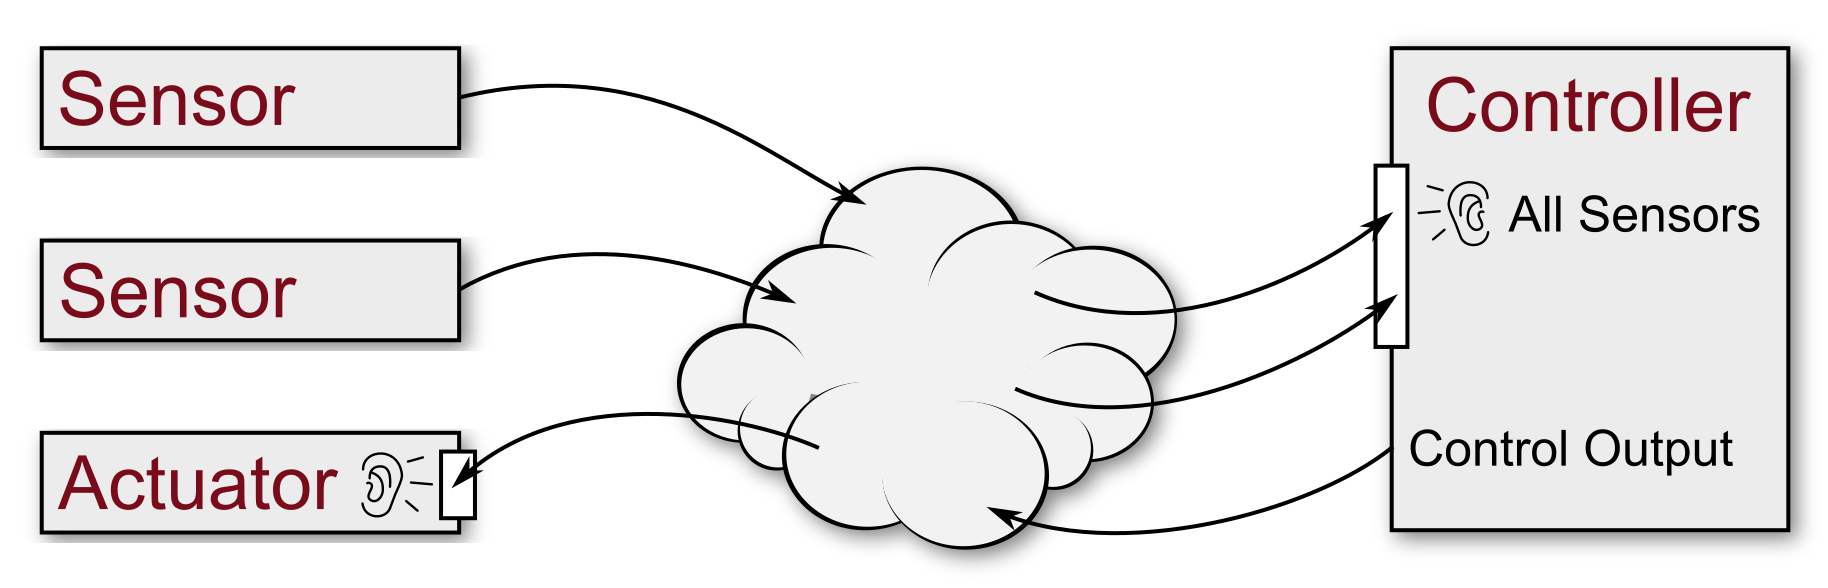
\includegraphics[width=0.62\textwidth]{messaging-scheme.png}
  \vspace{0.3cm}

  \begin{columns}[T]
    \column{0.48\textwidth}
    \small
    \begin{itemize}
      \item Every message carries a \alert{subject} (its name)
      \item Sources publish without knowing who listens
      \item Receivers subscribe to subjects, also with \alert{wildcards}
    \end{itemize}
    \column{0.48\textwidth}
    \small
    \begin{itemize}
      \item \textbf{Datapoint service}: simple \alert{get / set} of values
      \item Notifies on new values and on connection status
      \item Add a logger or plotter without touching the sensor
    \end{itemize}
  \end{columns}
\end{frame}

\begin{frame}{RPC: request and reply}
  \centering
  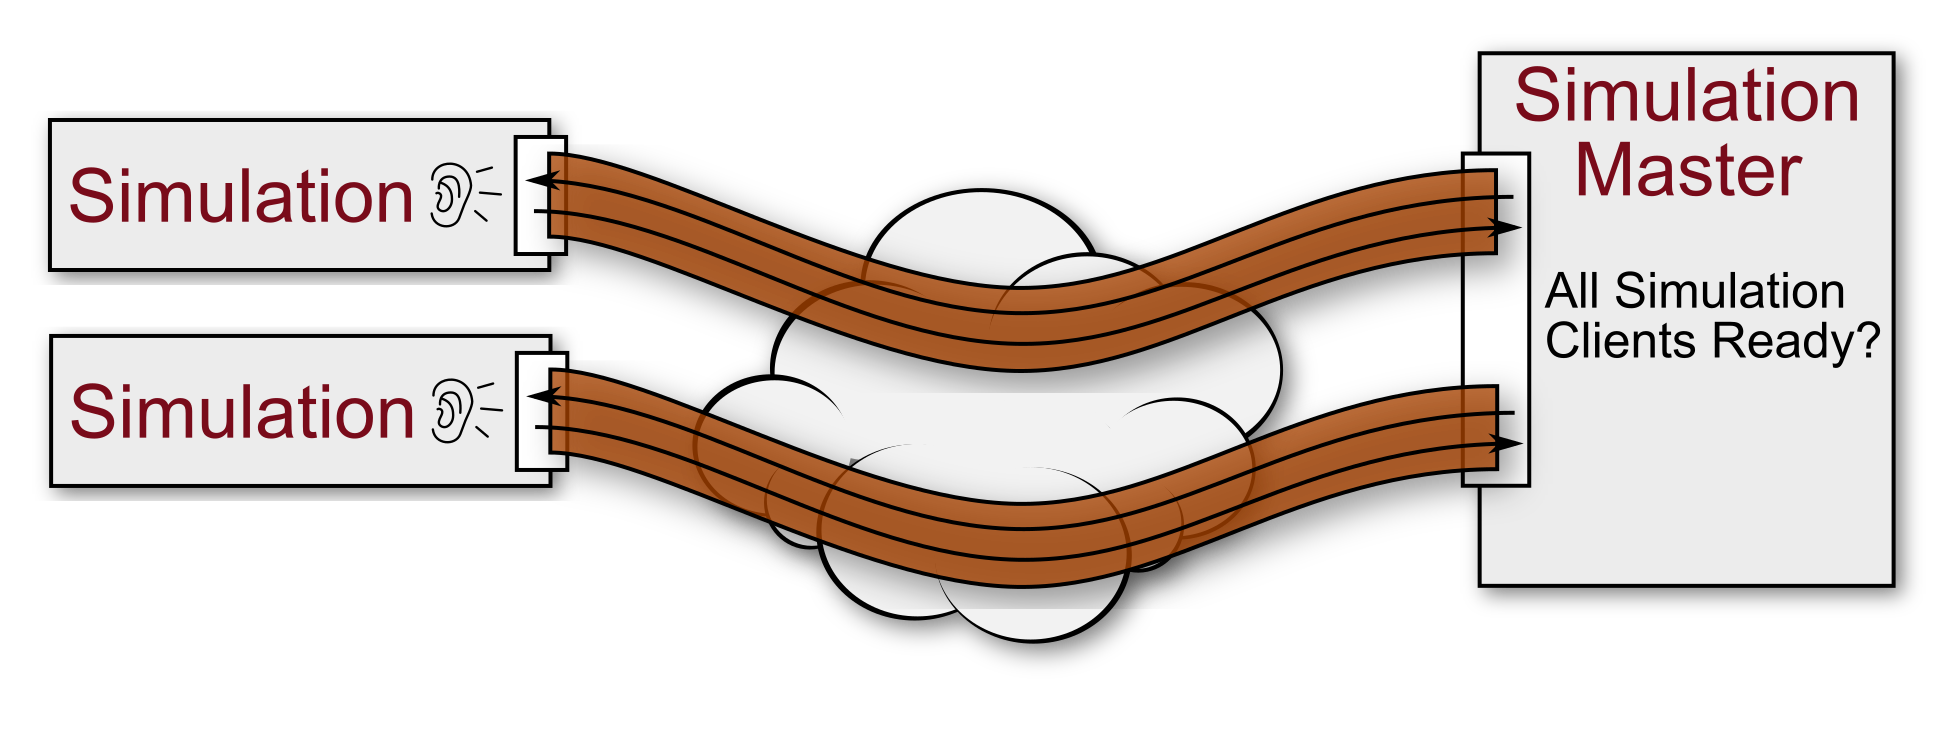
\includegraphics[width=0.7\textwidth]{rpc-scheme.png}
  \vspace{0.3cm}

  \begin{columns}[T]
    \column{0.48\textwidth}
    \small
    \begin{itemize}
      \item Requester picks the destination:\\ \alert{one client}, \alert{one group}, or \alert{everyone}
      \item Servers offer a fixed endpoint
    \end{itemize}
    \column{0.48\textwidth}
    \small
    \begin{itemize}
      \item Each reply is matched to its request
      \item Requester knows when \alert{all} answers are in, or when one is missing
    \end{itemize}
  \end{columns}
\end{frame}

\begin{frame}{Finding each other: addresses}
  \centering
  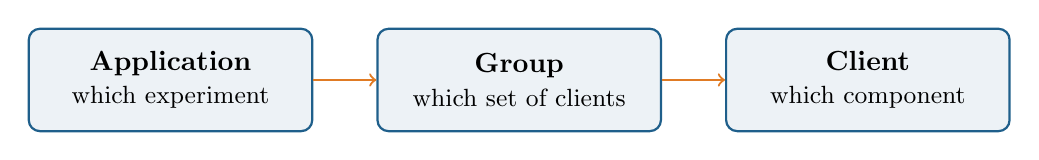
\begin{tikzpicture}[
      box/.style={rectangle, rounded corners, draw=llblue, thick, fill=llblue!8,
                  minimum width=3.6cm, minimum height=1.3cm, align=center}]
    \node[box] (app) {\textbf{Application}\\\small which experiment};
    \node[box, right=0.8cm of app] (grp) {\textbf{Group}\\\small which set of clients};
    \node[box, right=0.8cm of grp] (cli) {\textbf{Client}\\\small which component};
    \draw[->, thick, llorange] (app) -- (grp);
    \draw[->, thick, llorange] (grp) -- (cli);
  \end{tikzpicture}
  \vspace{0.8cm}

  \begin{itemize}
    \item Several experiments can share one broker in parallel
    \item RPC targets map directly onto this: one client, a group, or all
    \item Common pitfall: two clients with different application names cannot see each other
  \end{itemize}
\end{frame}

\begin{frame}{Sync: why a common clock?}
  \begin{columns}[c]
    \column{0.5\textwidth}
    \begin{itemize}
      \item A grid simulation, a controller and a real inverter must agree on \alert{what time it is}
      \item Without sync, each runs at its own pace and results drift apart
      \item The \textbf{sync host} is a stand-alone client that keeps everyone on one time
    \end{itemize}
    \column{0.46\textwidth}
    \begin{block}{The scenario file sets}
      \begin{itemize}
        \item Start and end time
        \item Step size
        \item Mode: simulation or emulation
        \item Settings for each participating client
      \end{itemize}
    \end{block}
  \end{columns}
\end{frame}

\begin{frame}{Sync: one step at a time}
  \centering
  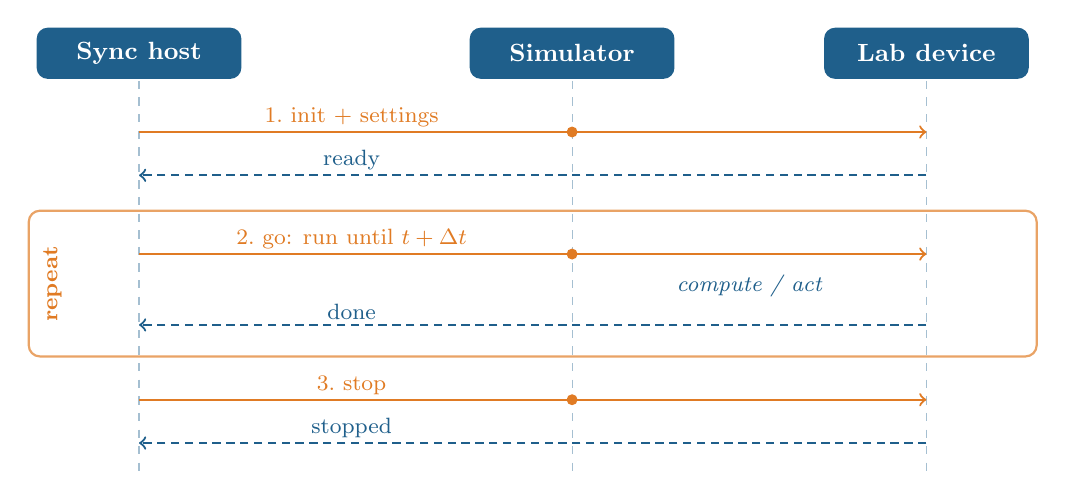
\begin{tikzpicture}[
      lane/.style={draw=llblue!40, dashed},
      act/.style={rectangle, rounded corners, fill=llblue, text=white, minimum width=2.6cm, minimum height=0.65cm, font=\small\bfseries},
      req/.style={->, thick, llorange},
      rep/.style={->, thick, llblue, densely dashed},
      lbl/.style={font=\footnotesize, above, inner sep=1.5pt},
      dot/.style={circle, fill=llorange, inner sep=1.4pt}]
    \node[act] at (0,0) {Sync host};
    \node[act] at (5.5,0) {Simulator};
    \node[act] at (10,0) {Lab device};
    \foreach \x in {0,5.5,10} \draw[lane] (\x,-0.35) -- (\x,-5.3);
    % init
    \draw[req] (0,-1.0) -- node[lbl, pos=0.27]{1.\ init + settings} (10,-1.0);
    \node[dot] at (5.5,-1.0) {};
    \draw[rep] (10,-1.55) -- node[lbl, pos=0.73]{ready} (0,-1.55);
    % loop
    \draw[llorange!70, thick, rounded corners] (-1.4,-2.0) rectangle (11.4,-3.85);
    \node[font=\footnotesize\bfseries, text=llorange, rotate=90] at (-1.1,-2.93) {repeat};
    \draw[req] (0,-2.55) -- node[lbl, pos=0.27]{2.\ go: run until $t+\Delta t$} (10,-2.55);
    \node[dot] at (5.5,-2.55) {};
    \node[font=\footnotesize\itshape, text=llblue] at (7.75,-2.95) {compute / act};
    \draw[rep] (10,-3.45) -- node[lbl, pos=0.73]{done} (0,-3.45);
    % stop
    \draw[req] (0,-4.4) -- node[lbl, pos=0.27]{3.\ stop} (10,-4.4);
    \node[dot] at (5.5,-4.4) {};
    \draw[rep] (10,-4.95) -- node[lbl, pos=0.73]{stopped} (0,-4.95);
  \end{tikzpicture}
  \vspace{0.2cm}

  \small The next step starts only when \alert{every} client has replied.\\
  Measured values flow as messages, independently of the steps.
\end{frame}

\begin{frame}{Sync: simulation vs.\ emulation}
  \begin{columns}[T]
    \column{0.48\textwidth}
    \begin{block}{Simulation mode}
      \begin{itemize}
        \item Next step starts as soon as all clients are done
        \item Can run \alert{faster} (or slower) than real time
        \item For pure software setups
      \end{itemize}
    \end{block}
    \column{0.48\textwidth}
    \begin{block}{Emulation mode}
      \begin{itemize}
        \item Steps are paced to the \alert{wall clock}
        \item Needed as soon as \alert{real hardware} is in the loop
        \item Clients must answer within the step, or the host reports it
      \end{itemize}
    \end{block}
  \end{columns}
  \vspace{0.3cm}
  \centering
  \small Rule of thumb: the step size must be longer than your slowest component needs per step.
\end{frame}

% ---------------------------------------------------------------- 5 Toolbox
\begin{frame}{A ready-made toolbox}
  \centering
  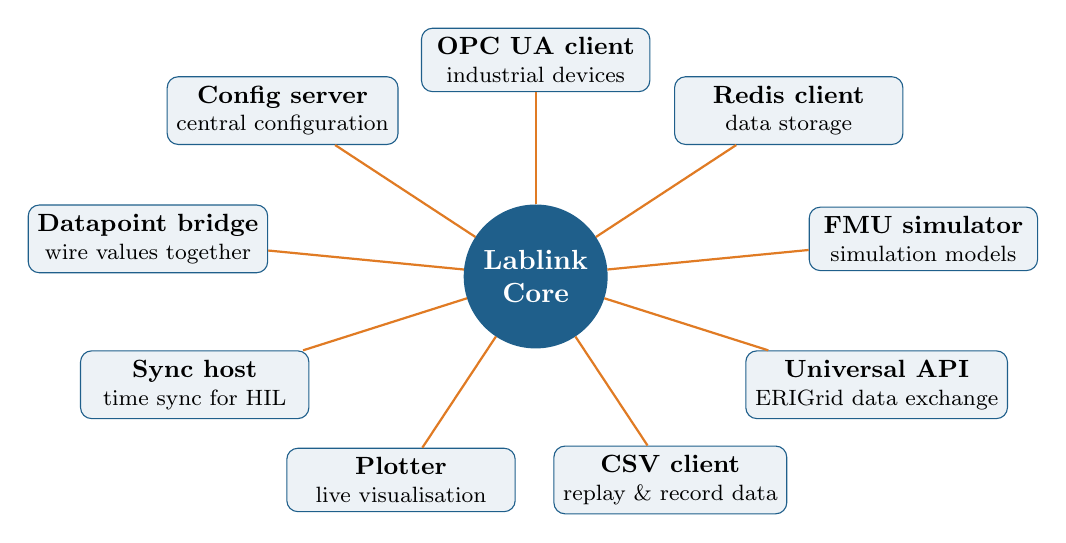
\begin{tikzpicture}[
      core/.style={circle, draw=llblue, fill=llblue, text=white, thick,
                   minimum size=1.8cm, align=center, font=\bfseries},
      cl/.style={rectangle, rounded corners, draw=llblue, fill=llblue!8,
                 minimum width=2.9cm, minimum height=0.8cm, align=center, font=\small}]
    \node[core] (c) {Lablink\\Core};
    \foreach \ang/\name/\what in {
        90/OPC UA client/industrial devices,
        50/Redis client/data storage,
        10/FMU simulator/simulation models,
        -30/Universal API/ERIGrid data exchange,
        -70/CSV client/replay \& record data,
        -110/Plotter/live visualisation,
        -150/Sync host/time sync for HIL,
        170/Datapoint bridge/wire values together,
        130/Config server/central configuration}{
      \node[cl] (n\ang) at ({5.0*cos(\ang)},{2.75*sin(\ang)}) {\textbf{\name}\\[-1pt]\footnotesize\what};
      \draw[llorange, thick] (c) -- (n\ang);
    }
  \end{tikzpicture}
\end{frame}

% ---------------------------------------------------------------- Config server
\begin{frame}{Configuration server: one place for every setup}
  \begin{columns}[c]
    \column{0.5\textwidth}
    \centering
    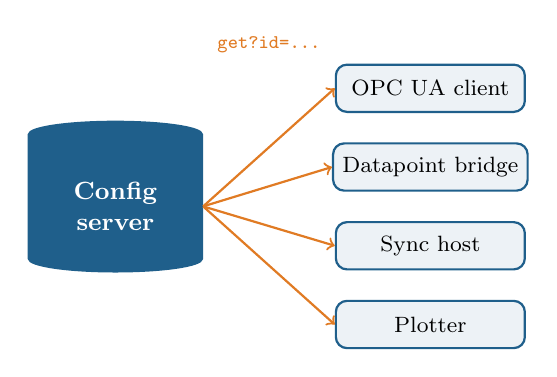
\begin{tikzpicture}[
        srv/.style={cylinder, shape border rotate=90, aspect=0.25, draw=llblue, thick,
                    fill=llblue, text=white, minimum width=2.2cm, minimum height=1.9cm,
                    align=center, font=\small\bfseries},
        cl/.style={rectangle, rounded corners, draw=llblue, thick, fill=llblue!8,
                   minimum width=2.4cm, minimum height=0.6cm, font=\footnotesize},
        ln/.style={<-, thick, llorange}]
      \node[srv] (s) at (0,0) {Config\\server};
      \foreach \y/\n [count=\i] in {1.5/OPC UA client, 0.5/Datapoint bridge, -0.5/Sync host, -1.5/Plotter}{
        \node[cl] (c\i) at (4.0,\y) {\n};
        \draw[ln] (c\i.west) -- (s.east);
      }
      \node[font=\scriptsize\ttfamily, text=llorange] at (1.95,2.05) {get?id=\dots};
    \end{tikzpicture}

    \column{0.48\textwidth}
    \small
    \begin{itemize}
      \item Stores all configurations of an experiment in \alert{one database file}
      \item Each client fetches its settings via a simple link:\\
        {\scriptsize\texttt{localhost:10101/get?id=demo.plotter}}
      \item A \alert{web browser} lists and shows all entries
      \item Settings files, JSON, or Python scripts that generate them
      \item Copy one file to \alert{share or archive} a lab setup
    \end{itemize}
  \end{columns}
\end{frame}

% ---------------------------------------------------------------- Datapoint bridge
\begin{frame}[fragile]{Datapoint bridge: wiring without code}
  \begin{columns}[c]
    \column{0.54\textwidth}
    \centering
    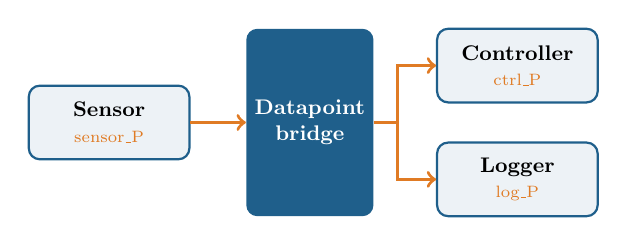
\begin{tikzpicture}[scale=0.85, every node/.style={transform shape},
        cl/.style={rectangle, rounded corners, draw=llblue, thick, fill=llblue!8,
                   minimum width=2.4cm, minimum height=1.1cm, align=center, font=\small},
        br/.style={rectangle, rounded corners, fill=llblue, text=white,
                   minimum width=1.9cm, minimum height=2.8cm, align=center, font=\small\bfseries},
        ln/.style={->, very thick, llorange}]
      \node[cl] (src) at (0,0) {\textbf{Sensor}\\\scriptsize\color{llorange}sensor\_P};
      \node[br] (b) at (3,0) {Datapoint\\bridge};
      \node[cl] (d1) at (6.1,0.85) {\textbf{Controller}\\\scriptsize\color{llorange}ctrl\_P};
      \node[cl] (d2) at (6.1,-0.85) {\textbf{Logger}\\\scriptsize\color{llorange}log\_P};
      \draw[ln] (src) -- (b);
      \draw[ln] (b.east) -- ++(0.35,0) |- (d1.west);
      \draw[ln] (b.east) -- ++(0.35,0) |- (d2.west);
    \end{tikzpicture}
    \vspace{0.4cm}

    \footnotesize
\begin{verbatim}
"Connections": [
  { "From": "sensor_P", "To": "ctrl_P" },
  { "From": "sensor_P", "To": "log_P"  }
]
\end{verbatim}

    \column{0.43\textwidth}
    \small
    \begin{itemize}
      \item Connects \alert{datapoints} of existing clients: new value at the source $\rightarrow$ written to the destination
      \item Wiring lives in a \alert{configuration file}, not in the clients
      \item Each link is \alert{one-way}; one source can feed several destinations
      \item Both ends need the \alert{same data type} (number, true/false, text, \dots)
      \item An unreachable destination is skipped and logged; the others keep receiving data
    \end{itemize}
  \end{columns}
\end{frame}

% ---------------------------------------------------------------- OPC UA
\begin{frame}{OPC UA client: speak the language of automation}
  \centering
  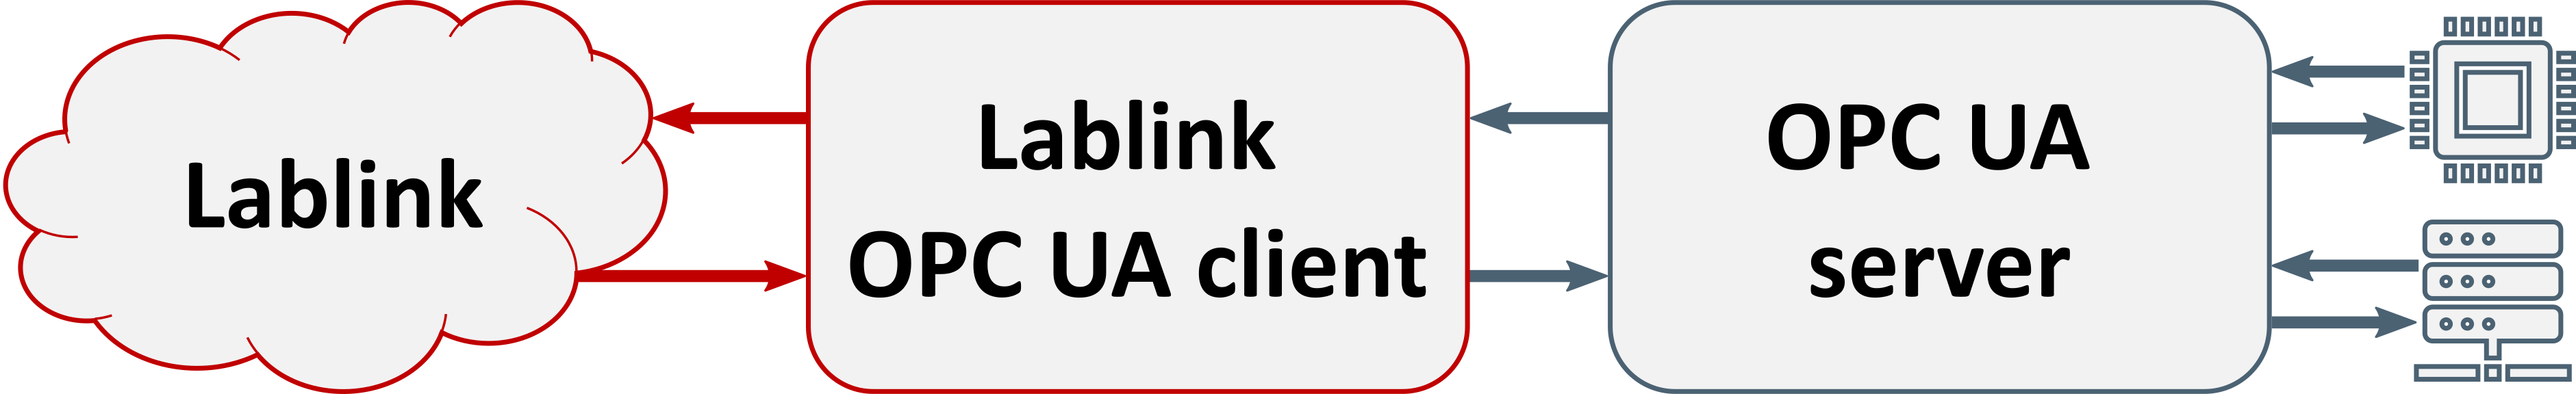
\includegraphics[width=0.75\textwidth]{lablink-opcua-client-overview.png}
  \vspace{0.3cm}

  \begin{columns}[T]
    \column{0.48\textwidth}
    \footnotesize
    \begin{itemize}
      \item \textbf{OPC UA}: vendor-independent standard in industrial automation, found in PLCs, SCADA systems, inverters and many lab devices
      \item One client connects Lablink to \alert{any OPC UA server}
      \item Login with user name and password, or anonymous
    \end{itemize}
    \column{0.48\textwidth}
    \footnotesize
    \begin{itemize}
      \item Lablink values are \alert{written} to server variables
      \item Changes on the server are \alert{sent} to Lablink (sampling interval configurable)
      \item Covers basic data types (numbers, true/false, text); a starting point for own extensions
    \end{itemize}
  \end{columns}
\end{frame}

% ---------------------------------------------------------------- Universal API
\begin{frame}[fragile]{Universal API client: lab signals via a web interface}
  \centering
  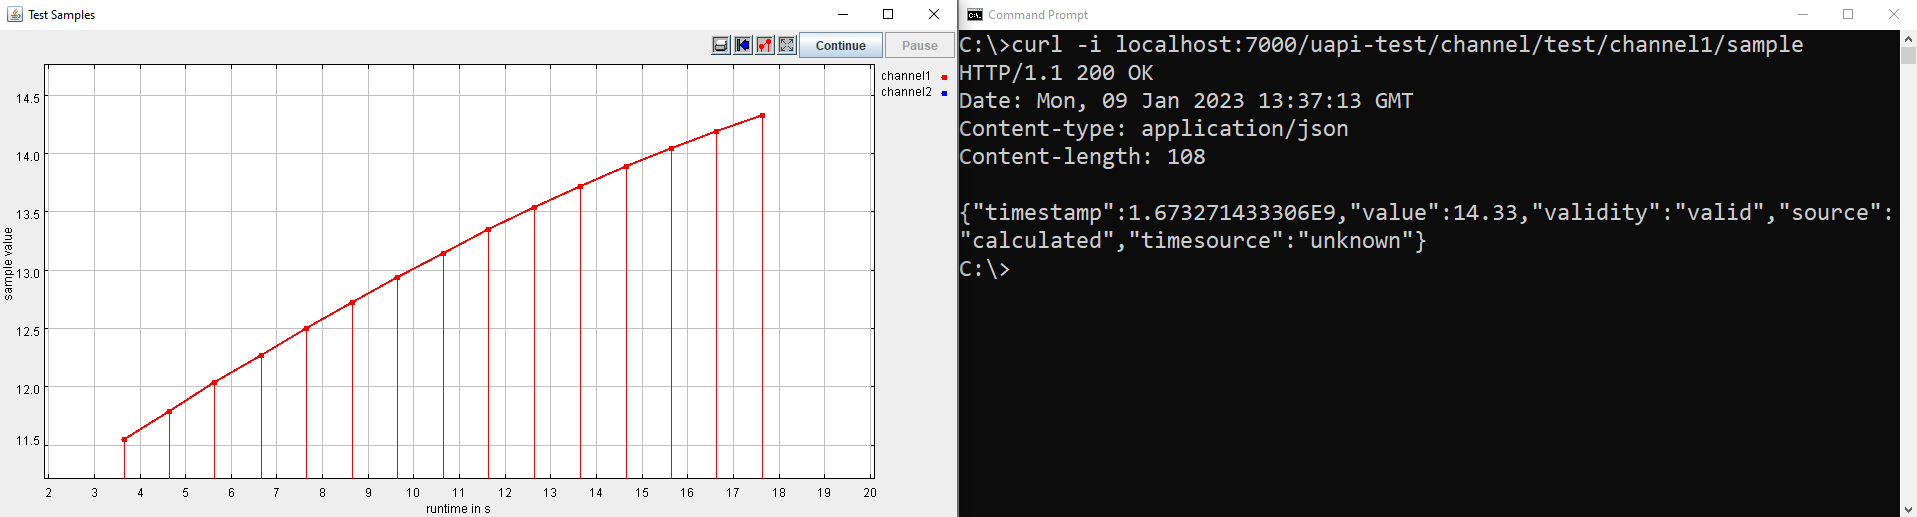
\includegraphics[width=0.62\textwidth]{example_read_signal_value.png}
  \vspace{0.2cm}

  \begin{columns}[T]
    \column{0.5\textwidth}
    \footnotesize
    \begin{itemize}
      \item Implements the \alert{ERIGrid Universal Data Exchange API}: a standardised \alert{REST} interface
      \item Anything that speaks HTTP can join: Python, MATLAB, a browser, a dashboard, a partner lab
      \item Channels are freely defined: readable / writable, data type, unit, allowed range
    \end{itemize}
    \column{0.46\textwidth}
    \scriptsize
\begin{verbatim}
GET  /channels                    list
GET  /channel/<id>/sample         read
PUT  /channel/<id>/sample         write
\end{verbatim}
    \small
    No Lablink code needed on the other side, just web requests.
  \end{columns}
\end{frame}

% ---------------------------------------------------------------- FMU
\begin{frame}{FMU simulator: bring models from any tool}
  \centering
  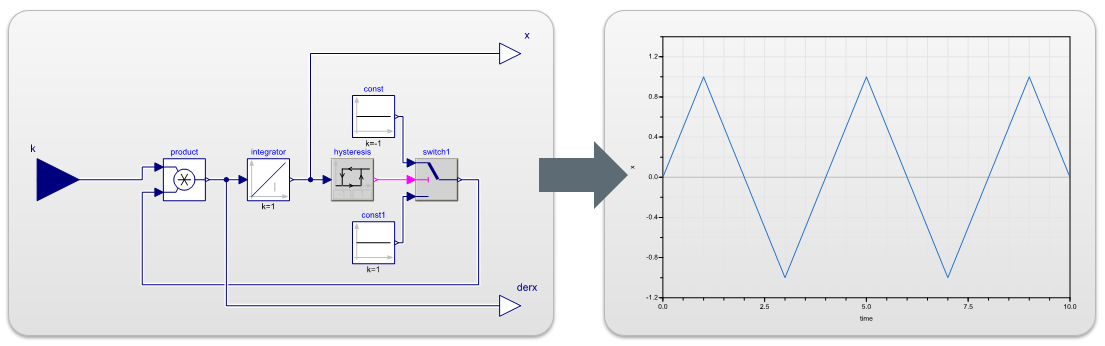
\includegraphics[width=0.55\textwidth]{fmu_sim_example.png}
  \vspace{0.2cm}

  \begin{columns}[T]
    \column{0.48\textwidth}
    \footnotesize
    \begin{itemize}
      \item \textbf{FMI}: open standard for exchanging simulation models; an \alert{FMU} is one packaged model
      \item Exported by many modelling tools, e.g.\ Modelica tools or Simulink
      \item The FMU simulator runs the model and links its inputs and outputs to Lablink
    \end{itemize}
    \column{0.48\textwidth}
    \footnotesize
    \begin{itemize}
      \item \alert{Fixed step}: strictly periodic, synchronised to real time
      \item \alert{Dynamic}: reacts to events in the model and to new inputs
      \item Models from different tools meet \alert{real hardware} in one setup
    \end{itemize}
  \end{columns}
\end{frame}

% ---------------------------------------------------------------- Plotter
\begin{frame}{Plotter: see what is happening, live}
  \centering
  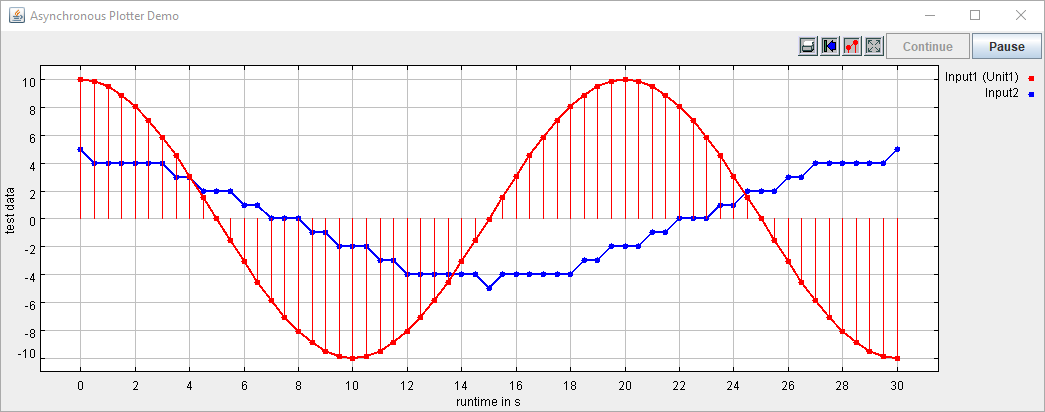
\includegraphics[width=0.52\textwidth]{plot.png}
  \vspace{0.2cm}

  \begin{columns}[T]
    \column{0.48\textwidth}
    \footnotesize
    \begin{itemize}
      \item Live graphs of any Lablink signals, continuously updated
      \item Pause and continue during a run
      \item Add or remove it without touching any other client
    \end{itemize}
    \column{0.48\textwidth}
    \footnotesize
    \begin{itemize}
      \item \alert{Asynchronous}: plots over wall-clock time
      \item \alert{Synchronous}: plots over simulation time, driven by the sync host
      \item Ideal for commissioning and quick sanity checks
    \end{itemize}
  \end{columns}
\end{frame}

% ---------------------------------------------------------------- 6 Example
\begin{frame}{Example: OPC UA test setup}
  \centering
  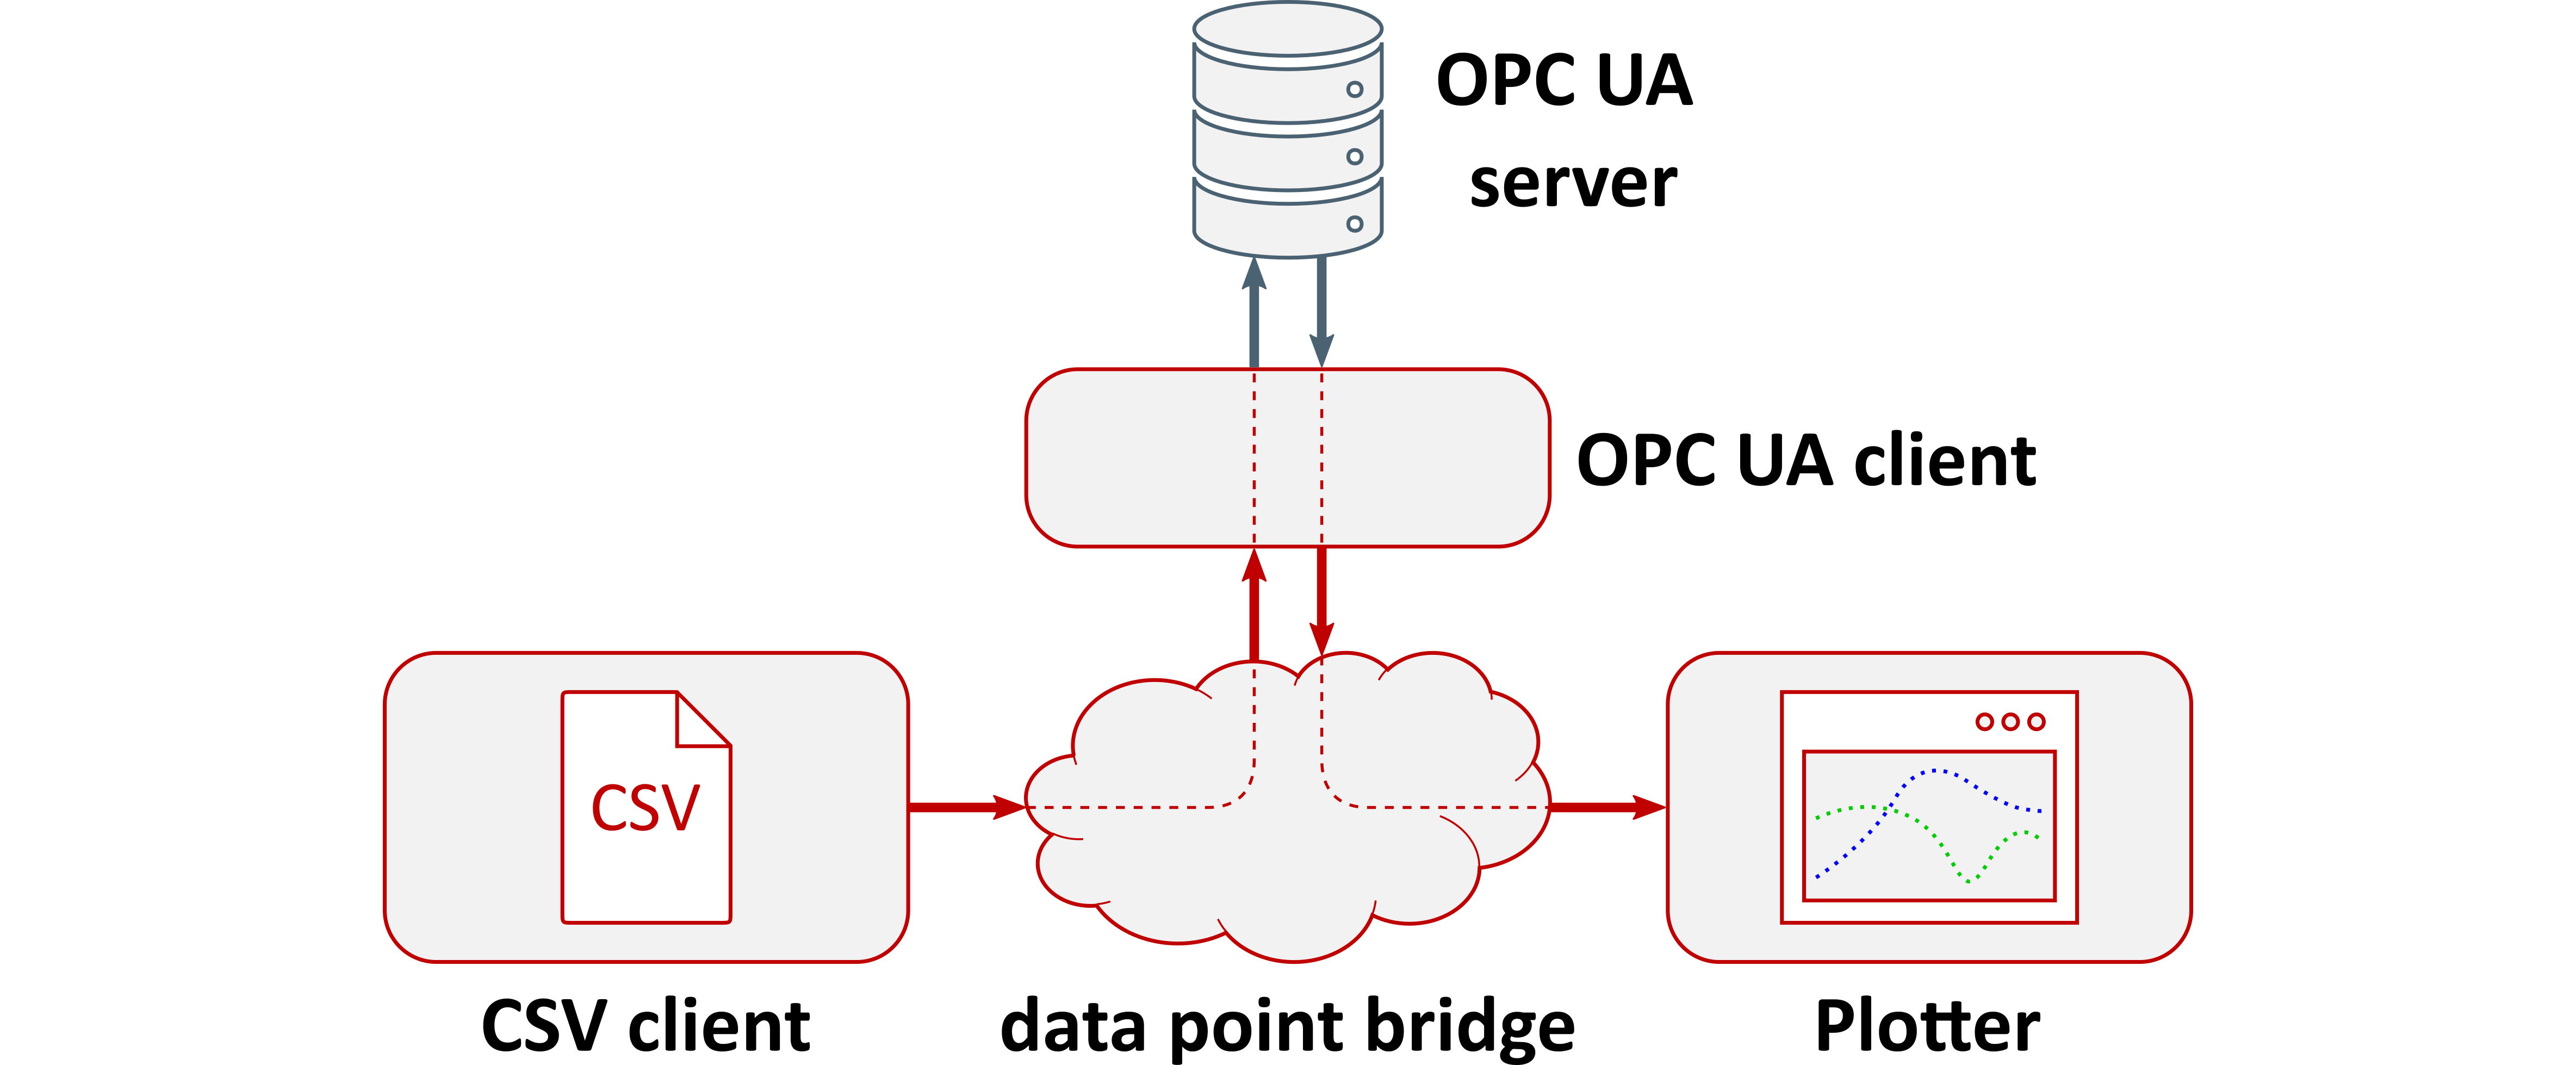
\includegraphics[height=0.45\textheight]{opcua-client-test-overview.png}
  \vspace{0.3cm}

  \small
  \begin{itemize}
    \item \textbf{CSV client} reads recorded data and sends it on
    \item \textbf{OPC UA client} writes the values to an OPC UA server and reads changes back
    \item \textbf{Plotter} shows everything live
  \end{itemize}
\end{frame}

\begin{frame}{Example: what you see}
  \centering
  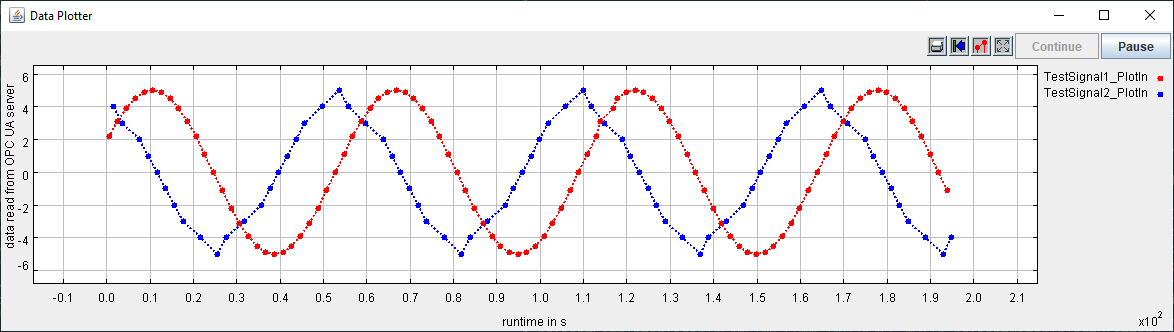
\includegraphics[width=0.9\textwidth]{opcua-client-test-plotter.png}
  \vspace{0.6cm}

  \begin{itemize}
    \item No custom code: three existing clients plus configuration files
    \item Replace the CSV source with a real device \alert{without changing} the rest
  \end{itemize}
\end{frame}

% ---------------------------------------------------------------- Scripting
\begin{frame}[fragile]{Automating configurations with Python}
  \begin{columns}[T]
    \column{0.53\textwidth}
    \centering
    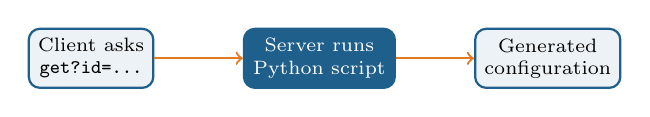
\begin{tikzpicture}[
        st/.style={rectangle, rounded corners, draw=llblue, thick, fill=llblue!8,
                   minimum height=0.75cm, align=center, font=\scriptsize},
        ln/.style={->, thick, llorange}]
      \node[st] (a) at (0,0) {Client asks\\\texttt{get?id=\dots}};
      \node[st, fill=llblue, text=white] (b) at (2.9,0) {Server runs\\Python script};
      \node[st] (c) at (5.8,0) {Generated\\configuration};
      \draw[ln] (a) -- (b); \draw[ln] (b) -- (c);
    \end{tikzpicture}
    \vspace{0.2cm}

    \fontsize{7}{8.5}\selectfont
\begin{verbatim}
class InverterSetup:
    def getJson(self):
        out = []
        for i in range(1, 9):    # 8 inverters
            out.append('{"Name":"P%d","DataType":"double",'
                       '"NodeIdString":"Inv%d.P"}' % (i, i))
        return HEADER + ", ".join(out) + "]}"
\end{verbatim}
    {\tiny\color{gray} simplified example}

    \column{0.45\textwidth}
    \footnotesize
    \begin{itemize}
      \item The config server can store a \alert{Python script} instead of fixed text
      \item On request it runs the script and hands the result to the client
      \item Loops instead of copy \& paste: \alert{8 or 80 devices}, same effort
      \item Change one parameter, regenerate all: ideal for \alert{test series}
      \item Also possible for the datapoint bridge; the config database itself can be filled by script
    \end{itemize}
  \end{columns}
\end{frame}

% ---------------------------------------------------------------- Containers
\begin{frame}[fragile]{Easy deployment with containers}
  \begin{columns}[T]
    \column{0.52\textwidth}
    \fontsize{6.6}{7.9}\selectfont
\begin{verbatim}
# docker-compose.yml (excerpt)
services:
  mqtt:
    image: eclipse-mosquitto:2
  lablink-config:
    image: ait1/lablink-config-server:latest
    volumes:
      - ./config/test-config.db:/app/config.db
    ports: ["10101:10101"]
  plotter:
    image: ait1/lablink-plotter:latest
    environment:
      LLCONFIG: http://lablink-config:10101/get?id=
      PLOT_CONFIG: demo.plotter
    ports: ["8080:8080"]
    depends_on: [mqtt, lablink-config]
\end{verbatim}

    \column{0.45\textwidth}
    \footnotesize
    \begin{itemize}
      \item Every Lablink client is a \alert{ready-made Docker image}: no Java build, nothing to install besides Docker
      \item \alert{One compose file} describes the whole setup: broker, config server, all clients
      \item \texttt{docker compose up} starts everything in the right order
      \item Plotter in the web browser; runs the same on laptop, lab PC or server
    \end{itemize}
    \vspace{0.1cm}
    \begin{block}{Complete experiment = 2 files}
      \texttt{docker-compose.yml} + config database
    \end{block}
  \end{columns}
\end{frame}

% ---------------------------------------------------------------- 7 Takeaways
\begin{frame}{Takeaways}
  \begin{columns}[T]
    \column{0.48\textwidth}
    \begin{block}{What you gain}
      \begin{itemize}
        \item Modular, reusable test setups
        \item Reproducible test runs
        \item Hardware and simulation in one loop
      \end{itemize}
    \end{block}
    \column{0.48\textwidth}
    \begin{block}{What you need}
      \begin{itemize}
        \item Docker (broker and clients come as ready-made images)
        \item Configuration of the clients, scriptable in Python
        \item Some IT support for the first setup
      \end{itemize}
    \end{block}
  \end{columns}
  \vspace{0.6cm}
  \centering
  \textbf{Start here:} \texttt{ait-lablink.readthedocs.io} \quad \textbullet \quad \texttt{github.com/ait-lablink}
\end{frame}

\begin{frame}[standout]
  Which manual coupling in your lab\\
  would you automate first?
\end{frame}

\end{document}
